\documentclass[11pt,a4paper]{report}

%------------ package pour langue fr ------
\usepackage[utf8]{inputenc}
\usepackage[french]{babel}
\usepackage[T1]{fontenc}
\usepackage{multicol}
%------------- for embedding images----------
\usepackage{graphicx} 
\usepackage{float}
\usepackage[export]{adjustbox}
\usepackage{amsfonts,epsfig,epstopdf,titling,url,array}

\usepackage{amsmath}
\usepackage{amssymb}
\usepackage{amsthm}
%--------- pour le style de la page ----------
%\usepackage[top=2cm, bottom=2cm, right=2cm, left=2cm]{geometry}
\usepackage[]{geometry}
\usepackage{setspace}
\setstretch{1,5}
%\usepackage{txfonts} //pour utiliser times new roman dans le document
\usepackage{fancyhdr}
\pagestyle{fancy}
\renewcommand\headrulewidth{1pt}
\fancyhead[L]{Bousbiat Hafsa}
\fancyhead[R]{Rapport Master}
%--------------------------- Sommaire ----------------------------%
\usepackage{hyperref}
\usepackage{amssymb}
\usepackage{natbib}
\theoremstyle{definition}
		\newtheorem{defn}{Definition}[section]
		\newtheorem{conj}{Conjecture}[section]
		\newtheorem{exmp}{Example}[section]
\begin{document}

%Page de garde (page de titre)							Obligatoire

\begin{titlepage}

\newgeometry{top=0mm,right=20mm,left=20mm,bottom=0mm}



	%--------------------  Entete de l'Ecole ----------------------%

	\begin{figure}[t]
		
\includegraphics[scale=0.75]{./ressources/image/ESI.png}\\[0.6in]
	\end{figure}
	
	
	
	%--------------------------------------------------------------%
	\begin{center}
	
	%------------------------  Le sujet ---------------------------%
		\LARGE \textbf{ Mémoire}\\
		\Large{
			Pour Obtention du diplôme de Master En Informatique\\
			\textbf{Option : Système Informatique (SIQ)}
			%\textsc thèse D'Ingéniorat En Informatique sous le thème :
		}\\[0.2in]
		\huge {
		\rule{\linewidth}{.5pt}
			\textbf{
				Étude et classification des méthodes de compression de graphe par extraction de motifs et k2-trees
			} 
			\rule{\linewidth}{.5pt}
		}\\[0.5in]
		\Large
	%--------------------------------------------------------------%	
	
	%-------------------------  Mon nom ---------------------------%
	\textbf{Réaliser par:}\\
	\begin{multicols}{2}
			\Large 	Mlle. Hafsa Bousbiat\\
			\large eh\_bousbiat@esi.dz\\
			ESI\\
		\columnbreak
 			\Large Mlle. Sana Ihadadene\\
			\large es\_ihadadene@esi.dz\\
			ESI \\
		
	\end{multicols} 
	
	\vskip 0.1in
	%--------------------------------------------------------------%	

	%-----------------------  Encadreures -------------------------%
	 \textbf{Encadrer par:}\\
	 
	 \begin{multicols}{2}
			\Large 	Dr. Karima Amrouche\\
			\large k\_amrouche@esi.dz\\
			ESI\\
		\columnbreak
 			\Large Dr. Hamida Seba\\
			\large hamida.seba@univ-lyon1.fr\\
			Université de Lyon \\
	\end{multicols}
	
	%--------------------------------------------------------------%	
	
	\small
	\vskip 0.3in
	Octobre 2018 \\
	Année Universitaire: 2018-2019\\
	
	\end{center}		
\restoregeometry
\end{titlepage}

%Remerciements											Obligatoire
\begin{center}
	\par
	\textit{
		\vskip 1in
		\Huge 
			Remerciement \\[0.5in]
			\addcontentsline{toc}{chapter}{\numberline{}Remerciement}
	}
\end{center}
	\par
  Nous tenons d'abord à exprimer notre gratitude à l'égard de nos encadrants, Madame Seba
Hamida, Madame Amrouche Karima et Monsieur Mohammed pour leur précieuse	aide, leur judicieux conseils  et pour le temps qu'ils nous ont consacré tout au long de ce PFE.\\


Nous remercions également toute l'équipe pédagogique de l'École Nationale
Supérieure d'Informatique, et à leur tète les enseignants pour la richesse et la qualité de la formation qu'ils nous ont offert tout au long de notre cursus.\\


Nous tenons à remercier les membres du jury qui nous ont fait l’honneur d’accepter de juger
cet humble travail.\\


Enfin, nous adressons nos plus sincères remerciements à tous nos proches et amis, qui nous ont toujours encouragée au cours de la réalisation de ce mémoire.
Merci à tous et à toutes.

\newpage
 


%Résumé												Obligatoire
\begin{center}
	\par
	\textbf{
		\vskip 0.5in
		\LARGE 
			Résumé \\[0.15in]
			\addcontentsline{toc}{chapter}{\numberline{}Résumé}
	}
\end{center}
	\par
    Lorem ipsum dolor sit, amet consectetur adipisicing elit. Nostrum tempore ea fugiat numquam autem saepe quas porro vitae? Fugit commodi tempore voluptate sint fugiat, possimus optio ad! Pariatur, obcaecati quidem.
Lorem ipsum dolor, sit amet consectetur adipisicing elit. Neque excepturi ducimus accusantium eius voluptatibus, quod velit, explicabo tenetur aliquid ipsam sapiente. Quibusdam quis ullam, saepe numquam molestias nobis recusandae labore?    Lorem ipsum dolor sit, amet consectetur adipisicing elit. Nostrum tempore ea fugiat numquam autem saepe quas porro vitae? Fugit commodi tempore voluptate sint fugiat, possimus optio ad! Pariatur, obcaecati quidem.
Lorem ipsum dolor, sit amet consectetur adipisicing elit. Neque exceptu 

\begin{center}
	\par
	\textbf{
		\vskip 0.5in
		\LARGE 
			Abstract \\[0.15in]
	}
\end{center}
	\par
    Lorem ipsum dolor sit, amet consectetur adipisicing elit. Nostrum tempore ea fugiat numquam autem saepe quas porro vitae? Fugit commodi tempore voluptate sint fugiat, possimus optio ad! Pariatur, obcaecati quidem.
Lorem ipsum dolor, sit amet consectetur adipisicing elit. Neque excepturi ducimus accusantium eius voluptatibus, quod velit, explicabo tenetur aliquid ipsam sapiente. Quibusdam quis ullam, saepe numquam molestias nobis recusandae labore?    Lorem ipsum dolor sit, amet consectetur adipisicing elit. Nostrum tempore ea fugiat numquam autem saepe quas porro vitae? Fugit commodi tempore voluptate sint fugiat, possimus optio ad! Pariatur, obcaecati quidem.
Lorem ipsum dolor, sit amet consectetur adipisicing elit. Neque exceptu

\newpage

%Sommaire (Table des matières)							Obligatoire
\tableofcontents
\newpage

%Liste des figures										Selon besoin
\listoffigures
\addcontentsline{toc}{chapter}{\numberline{}Liste des figures}
\cleardoublepage

%Liste des tableaux										Selon besoin

\listoftables
\addcontentsline{toc}{chapter}{\numberline{}Liste des tableaux}
\cleardoublepage

%Introduction (début de la pagination)					bligatoire


\part{Introduction} 


%---->chapitre 01 :« cadrage du projet »
	\chapter{ Théorie des graphes}
	
%---->Introduire les graphe la motivation deriere leurs utilisation pour modeliser	
	
	\section{Graphe non orienté}
		\subsection{Définitions et généralités}
		\subsection{Représentation graphique}
		\subsection{Propriété d'un graphe} %% a revoir 
			\subsubsection{Degré d'un graphe:} %% esk le degre de graphe ou de neoud
			\subsubsection{Rayon d'un graphe:}
			%%%% A revoire d'autre memoire sur Graph theory
			
	
	
	
	
		\subsection{Définitions et généralités}
		Un graphe orienté G est la donnée d'un couple (V , E) où
		V est un ensemble fini dont les éléments sont appelés les sommets de G et 
		E  $\subset$ V x V est un ensemble de couples ordonnés de sommets dits arcs ou arêtes \citep{muller}. G est appelé dans ce cas digraphe (directed graph).\\
		 Pour tout arc e = ( $v_{i}$ , $v_{j}$) $\in$ E :
		 \begin{itemize}  
			\item $v_{i}$ est dit extrémité initiale ou origine de e et $v_{j}$ est l'extrémité finale de e \citep{muller}.
			
			\item $v_{i}$ est le prédécesseur de $v_{j}$ et $v_{j}$ est le successeur de $v_{i}$ \citep{IUTLyonInformatique}.
			
			\item les sommets $v_{i}$ , $v_{j}$ sont des sommets adjacents \citep{Pres}.
			
			\item e est dit sortant en $v_{i}$ et incident en $v_{j}$ \citep{Pres}.
			
			\item e est appelé boucle si $v_{i}$ = $v_{j}$, i.e l'extrémité initiale et finale représente le même sommet \citep{IUTLyonInformatique}.
			
		\end{itemize}
		 
		
		\subsection{Représentation graphique}
		
		
		Un graphe G = (V , E) peut être projeter sur le plan en représentant:
		\begin{itemize} 
		\item Dans un premier temps les nœuds $v_{i}$ $\in$ V par des points disjoints du plan.
		\item Et dans un second temps les arêtes e = ( $v_{i}$ , $v_{j}$) $\in$ E par des lignes orientées reliant par des flèches les deux extrémités de e. 
		\end{itemize}
		
		\textbf{Exemple:}
		
		Soit g = ($V_{1}$ , $E_{1}$) un digraphe tel que : $V_{1}$ = \{ 1,2,3,4 \} et  $E_{1}$ = \{(1,2),(1,3),(3,2),(3,4),(4,3)\}.
		
		Le représentation graphique de g est alors donné par le schéma de la figure \ref{grapheOr}.
	
		
			\begin{figure}[h]
			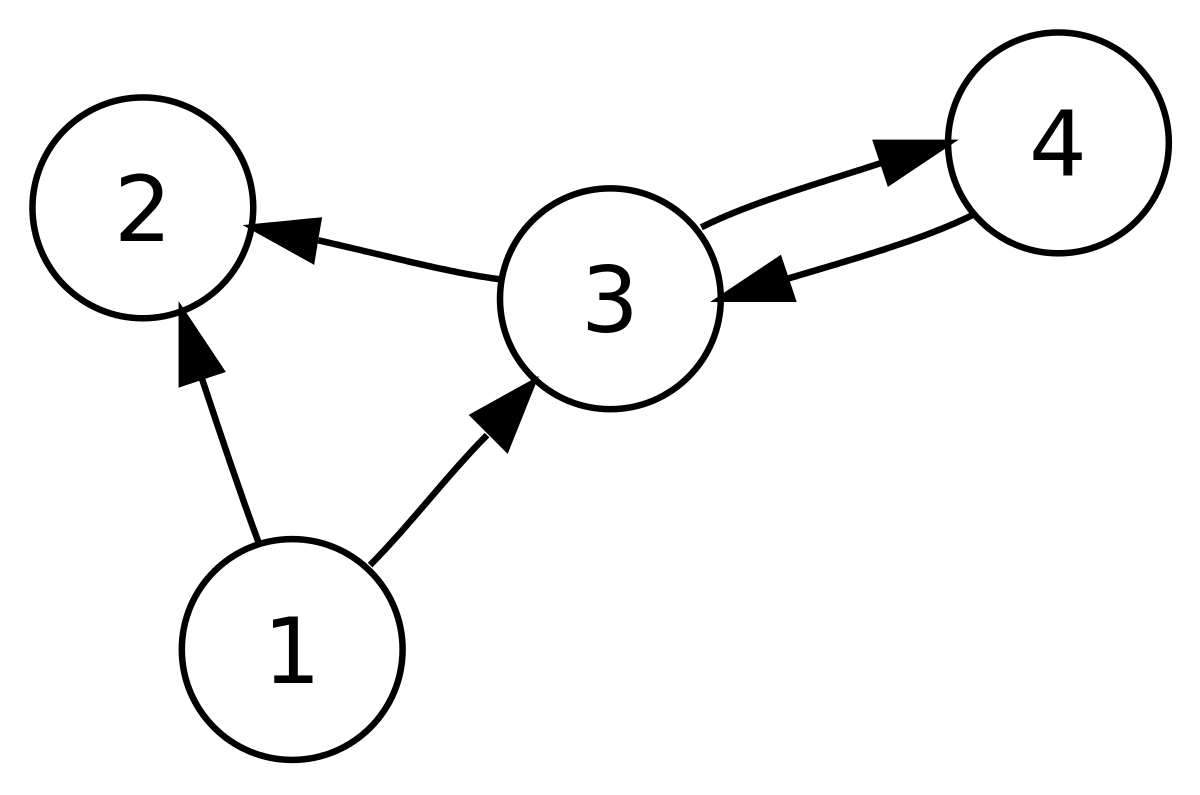
\includegraphics[scale=0.15,center]{./ressources/image/RepDiGraphe.png}
			\caption[Exemple de représentation graphique d'un digraphe.]{Exemple de représentation graphique d'un digraphe.}
			\label{grapheOr}
			\end{figure}
			
		
		\subsection{Quelques Propriétés:} %%% Arevoire 
			\begin{itemize}[label=$\circ$]
			\item\textbf{Ordre d'un digraphe:}
			est le nombre de sommets n = Card(V) \citep{DUT}.
			
			\item\textbf{taille d'un digraphe:} est le nombre d’arcs m = Card(A) \citep{DUT}.
			
			\item\textbf{Degré dans un digraphe:}
			Le degré d'un sommet $v_{i}$ $\in$ V dans un digraphe G=(V , E) est donnée par la formule :
			\begin{center}
				d($v_{i}$) = $d^+(v_{i}$) + $d^-(v_{i}$\\
			\end{center}			 
			 où $d^+(v_{i}$) est le nombre d'arcs sortants au sommet $v_{i}$ et est appelé degré extérieure et $d^-(v_{i}$) représente le nombre d'arcs incidents et est appelé degré intérieur \citep{muller}.
			 
			 \item\textbf{Voisinage dans un digraphe:}
			 Le voisinage d'un sommet $v_{i}$ $\in$ V, noté V($v_{i}$), dans un digraphe G = (V , E) est:
			 	\begin{center}
				V($v_{i}$) = succ($v_{i}$) $\bigcup$ pred($v_{i}$),
				\end{center}
				
				où succ($v_{i}$) est l'ensemble des successeurs de $v_{i}$ et pred($v_{i}$) est l'ensemble de ses prédécesseurs \citep{bac}, i.e le voisinage de $v_{i}$ est l'ensemble des sommets qui lui sont adjacents.
			
			\end{itemize}
			
	
	
			 
			
	\section{Type de graphe} %% classifier selon le type du graphe en entree
		\begin{defn}
			Here is a new definition
		\end{defn}
	
	\section{Représentation Structurelle d'un graphe}
		\subsection{Représentation par une matrice}
			\subsubsection{Matrice d'adjacence}
			\subsubsection{Matrice d'incidence}
		\subsection{Représentation par une liste}
			\subsubsection{Liste d'adjacence}
			\subsubsection{Liste d'incidence}
			
			
	\section{Les domaines d'application}
	

%---->chapitre 02 :« »
	\chapter{Compression de graphe}
	


%---->chapitre 03 :« Etude empirique »
	\chapter{chapitre 03: etude empirique}

%Conclusion Générale									Obligatoire
\part{Conclusion} 

%Références Bibliographiques (fin de la pagination)		Obligatoire

%Annexes													Selon besoin
Random citation \citep{seo2018effective} embeddeed in text.

Random citation \citep{brisaboa2009k} embeddeed in text.

\newpage
\bibliography{Bibliographie}
\bibliographystyle{apalike}

\end{document}

%\renewcommand{\thefigure}{\arabic{figure}}
%\setcounter{figure}{0}
%\begin{figure}[H]
%	\centering
%	\includegraphics[scale=1]{ressources/image/LAAS-2016.jpg}
%	\label{fig:figure1}
%	\caption{This is a teste of figure}
	
%\end{figure}








